% !TEX root = ../HPCA2016.tex
\section{Architecture}
\label{sec:Architecture}

Our clustered migration mechanism was carefully designed to address key challenges associated with the migration problem. In the remainder of this section, we present a complete description of our micro-architectural design, followed by a breakdown of all important design decisions made along with the challenge addressed by each one.

\subsection{Clustered Migration Architecture}

 Figure \ref{fig:architecture_complete} presents an overview of MemPod. MemPod's design was kept modular to facilitate system integration. A number of memory pods are injected between the LLC and the system's MCs. Each pod clusters a number of MCs and restricts migration  within the pod. To the rest of the system, pods are seen as MCs. With MemPod's transparent design, each pod will now be receiving all the requests originally addressed to any of the pod's MCs. 

A pod's operation when a memory request arrives would be to monitor the request, update any necessary migration-related counters and forward the request to the intended recipient MC. The migration logic within a pod does not need to be invoked during a response from any MC and could potentially be bypassed, saving some cycles. An obvious drawback of clustering MCs into pods is the serialization of potentially parallel requests to different MCs and as such, any counting scheme used by the pod -- as well as the actual forwarding of the request -- have to be as efficient as possible. 

\begin{figure}[h]
  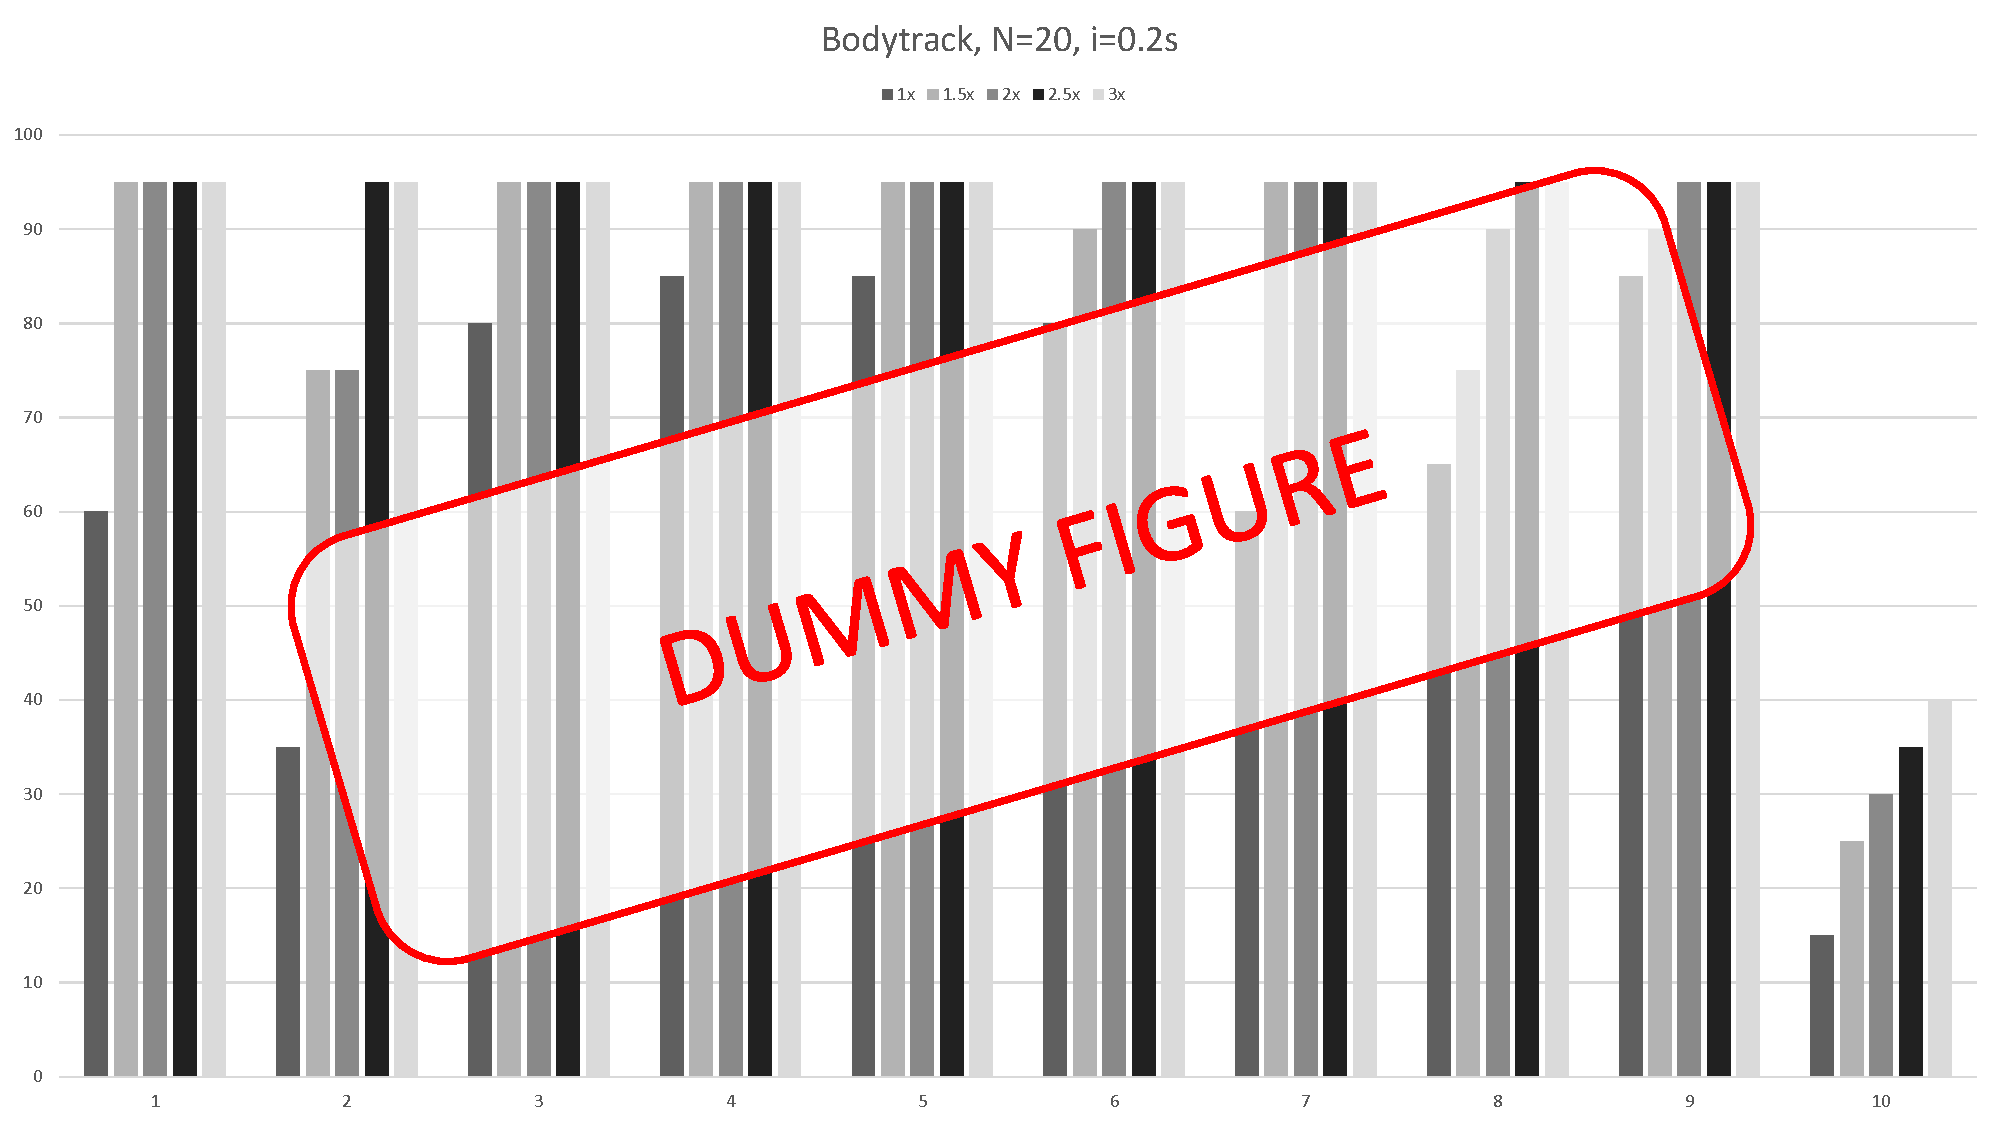
\includegraphics[width=0.46\textwidth]{figures/dummy.pdf}
  \caption{MemPod high-level architecture}
  \label{fig:architecture_complete}
\end{figure}

\begin{figure}[h]
  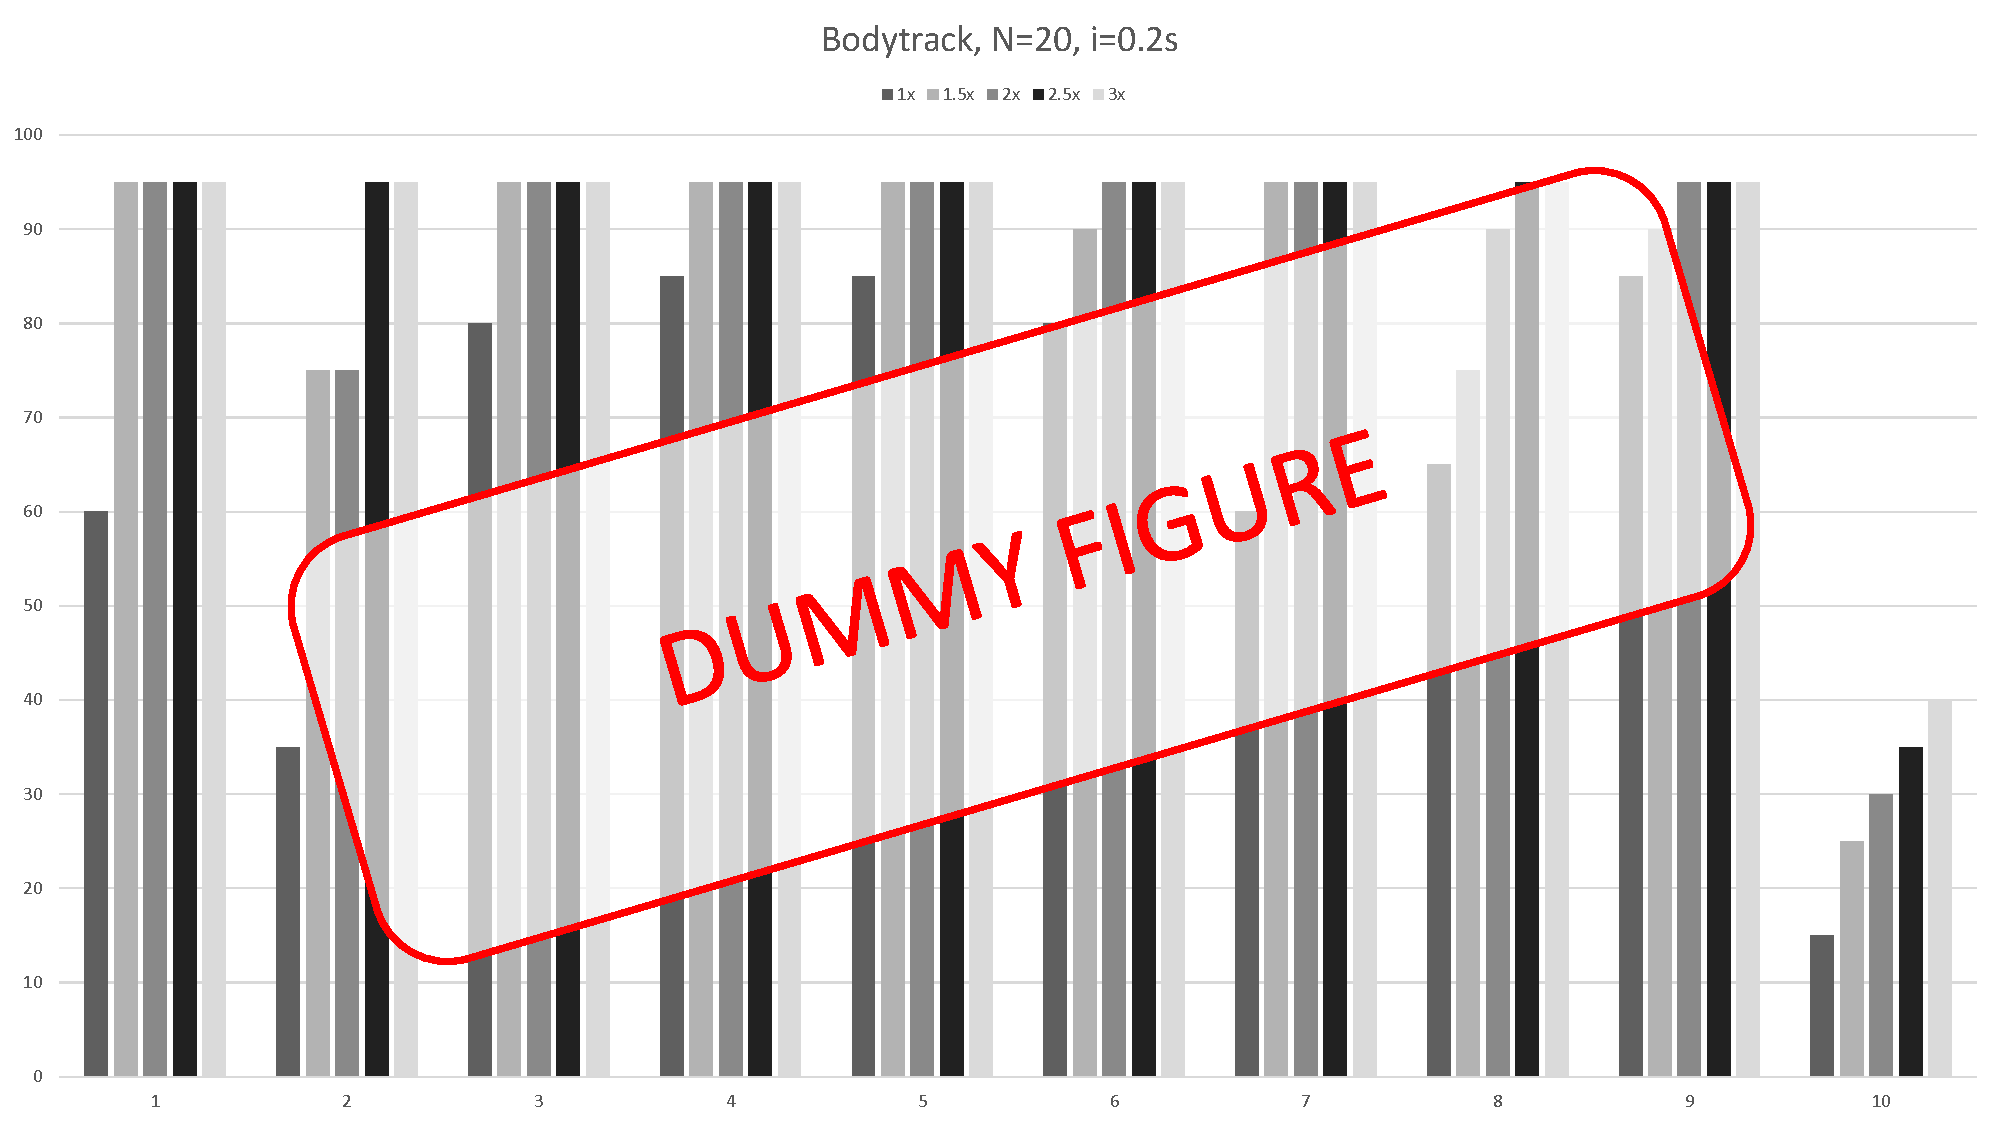
\includegraphics[width=0.46\textwidth]{figures/dummy.pdf}
  \caption{Major architectural Pod elements}
  \label{fig:architecture_pod}
\end{figure}

\subsubsection*{Memory Pod}
The major architectural elements of a Pod are presented in Figure \ref{fig:architecture_pod}. A Pod's remap structure includes the remap table as well as necessary decoding and hit detection logic. Counting logic is equally important for migration as the existence of a remap table and it's responsible for identifying the hot pages which will later be candidates for migration. Without reliable hot page detection, migration would be random and often counter-productive. Finally, migration logic is responsible for orchestrating a page swap between two MCs and updating the Pod's state.

During the design of a new system, the number of pods can vary arbitrarily given different constrains. A design with just one cluster would be equivalent to a centralized migration controller allowing any-to-any\footnote{Any-to-any Migration: Page migration without limits on source and destination. All MCs can migrate a page to any MC.} migration, while a design with a pod number equal to the number of MCs would imply that migration is disabled. The latter option would be completely redundant and is only used as an example. A reasonable number of Pods would be equal to the number of slow-memory MCs. In Figure \ref{fig:architecture_complete} we present a system with eight MCs for the fast, on-die stacked memory and four MCs for the slow off-chip memory. The use of four pods imposes few restrictions on migration possibilities, while forbiding migration between two slow-memory MCs. For the remainder of this paper, we set the number of pods to four.

The dollowing subsections provide detailed descriptions of all major elements of a migration management mechanism. We present MemPod's, THM's and HMA's approach to each element's design, as well as alternative designs. It's important to note that each of the following elements is independent from all the rest and future mechanisms could choose almost any element design combination in a plug-and-play fashion, with some exceptions. For example, the use of Majority Element Algorithm (MEA) activity tracking cannot work with threshold-based triggers.

\subsection{Decentralization of migration logic}

\subsection{Page Relocation and Remap Table Size}

Migration of memory pages can provide maximum benefits when no restrictions are imposed on the available migration locations. In other words, the optimal scenario for a migration policy would be the option of potentially filling the entire fast memory with migrated hot pages. On the other hand, more options require more bookkeeping and incur a higher cost. Flat address space memories do not have the luxury of a backing memory, like a 3D-stacked DRAM cache. Consequently, migrating a page implies swaping two pages to ensure the existence of exactly one copy for each of the participating pages. As such, migrating and swaping will be used interchangeably for the remainder of this paper.

A traditional remap table is a hash structure, indexed by a page's address and pointing to the migrated address if one exists. On a page migration, the remap table is updated to reflect the new address of a migrated pge. However, such a remap table is not enough when re-migration of pages is allowed. Figure \ref{fig:failed_remap} presents a scenario where a ''naive`` remap table fails. Figure \ref{fig:failed_remap}(i) shows the starting state of our memory before any migration, as well as the starting state of the remap table. For simplicity, we present the three memory locations needed by our example. Page 10 is assumed to be a fast memory page, while pages 100 and 200 are slow memory pages. The numbers inside the memory locations represent the content page's id. Figure \ref{fig:failed_remap}(ii) shows the state of memory and remap table after swaping pages 10 and 100. The content of page 10 is now page 100, and the content of page 100 is now 10. The remap table correctly states that requests to page 10 should be relayed to page 100 and vice versa.  Everything works as it should during this first migration, however Figure \ref{fig:failed_remap}(iii) shows the state after the second migration. Page 10 is now swaped with page 200. Such a migration would imply that page 100 (now held at 10) became cold and page 200 became hot. The contents are swaped and now page 10 holds page 200 and page 200 holds page 100. However, the state of the remap table is inconsistent. A request to page 10 would get forwarded to page 200, returning the wrong page.

The reason this remap table design fails is simply because pages are allowed to re-migrate -- like page 10 in our previous example -- while the remap table ''assumes`` the content held at a page address matches the page's ID.  There is only one solution to this problem: The migration logic needs to be aware of exactly where each page's contents are located at any given time. Such a requirement can be implemented in various ways:
\begin{enumerate}
	\item \textbf{Safe and slow:} Always restore a forwarded page's contents before it participates in a new migration. For such an implementation, hot page count will have to be kept based on the content page instead of the real page Id. In the earlier example in Figure \ref{fig:failed_remap}, the second migration of page 10 implies that page 100 is cold, but in order to offer page restoration support, the second swapping of page 10 will have to imply that page 10 is cold. The cold page (10) will be restored back to address 10 from 100 and then moved to its new location. It's a minor modification that does not affect any other aspect of a migration mchanism.
	\item \textbf{THM approach:}Migration is restricted in segments. In a memory configuration with a 1:8 fast:slow memory ratio, exactly 9 pages compete for a position at the one fast memory page available. This solution is elegant enough to allow re-migration without extremely high storage overhead, limiting however the migration potential of memory pages. If two or more hot pages coexist in a segment, only one can reside in fast memory at any given time.
	\item \textbf{HMA approach:} Any page can migrate to any other page address. The OS-based migration scheme imposes no limitations, since the OS takes care of updating the page tables and flush the TLB, however the cost of HMA's intervention and the penalties incurred from a cold TLB could sum up to very high values.
	\item \textbf{MemPod approach:} Migration is restricted within a Pod, but no location restrictions are applied. A Pod's remap table is extended with a second field that holds the content page's id. During the second migration in our previous example, the issue was caused because we updated the remap entry of the holding page (10) instead of the entry of the content page (100). An attempt to recursively follow the remap table's entries until we figure out which one we should update risks looping infinitely because of cycles (For Example if page 10 is re-migrated back to address 10). Even if a smart algorithm is utilized to delete entries of non-migrated pages, the complexity of the recursive algorithm will only be bounded by the size of the remap table since in the worst case the entire table will be traversed. Figure \ref{fig:correct_remap} shows the memory and remap table states after the same page mirations as in Figure \ref{fig:failed_remap}. At the end of the second migration, the states of memory and remap table are consistent. It's important to note that a remap table entry is now points to a pair of values: (1) \textit{relay address} (i.e. where is the requested page located) and (2)\textit{content address} (Which page is currently held).
\end{enumerate}

\TODO{Discuss the cost of MemPod and THM approach in terms of storage overhead. They should be similar.}

\begin{figure}[h]
  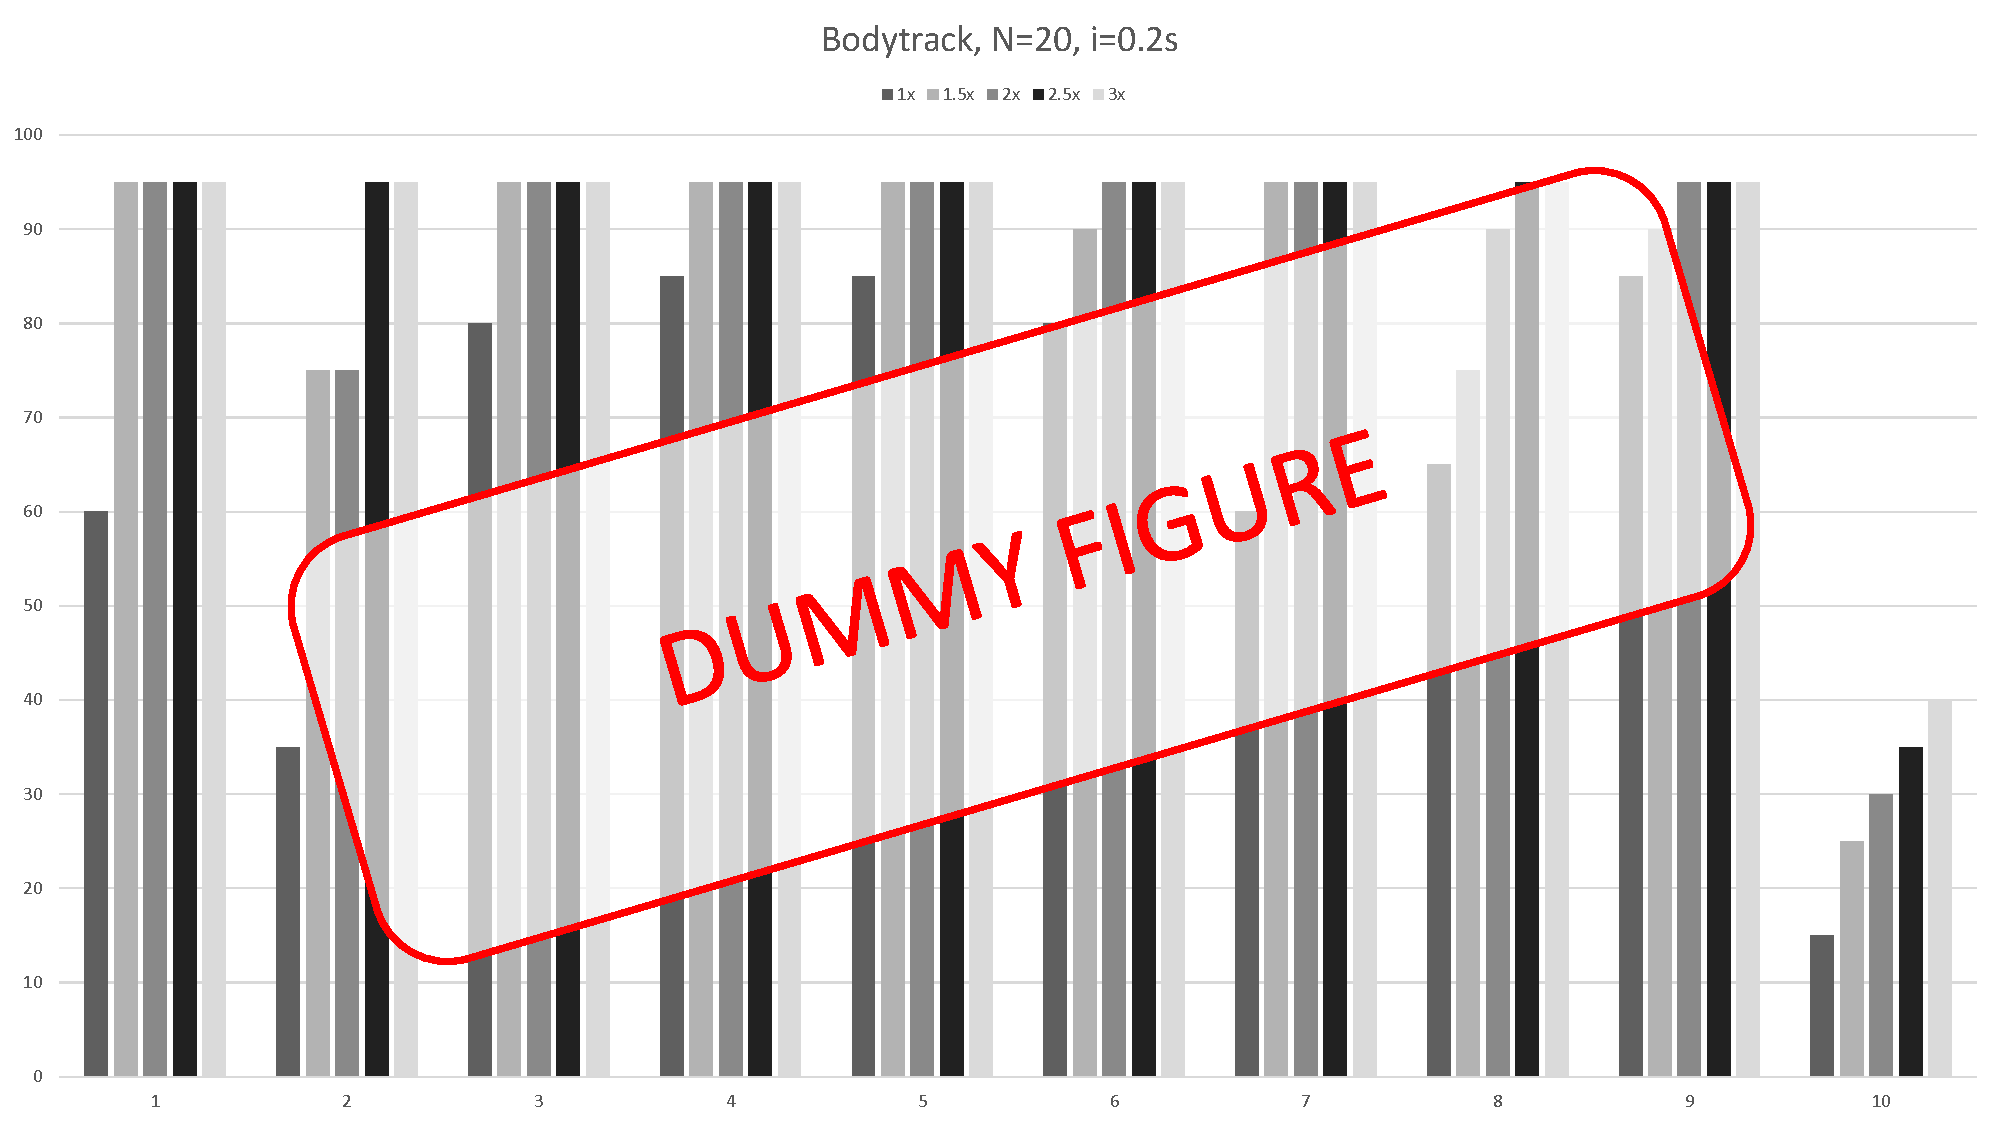
\includegraphics[width=0.46\textwidth]{figures/dummy.pdf}
  \caption{Naive remap table operation}
  \label{fig:failed_remap}
\end{figure}

\begin{figure}[h]
  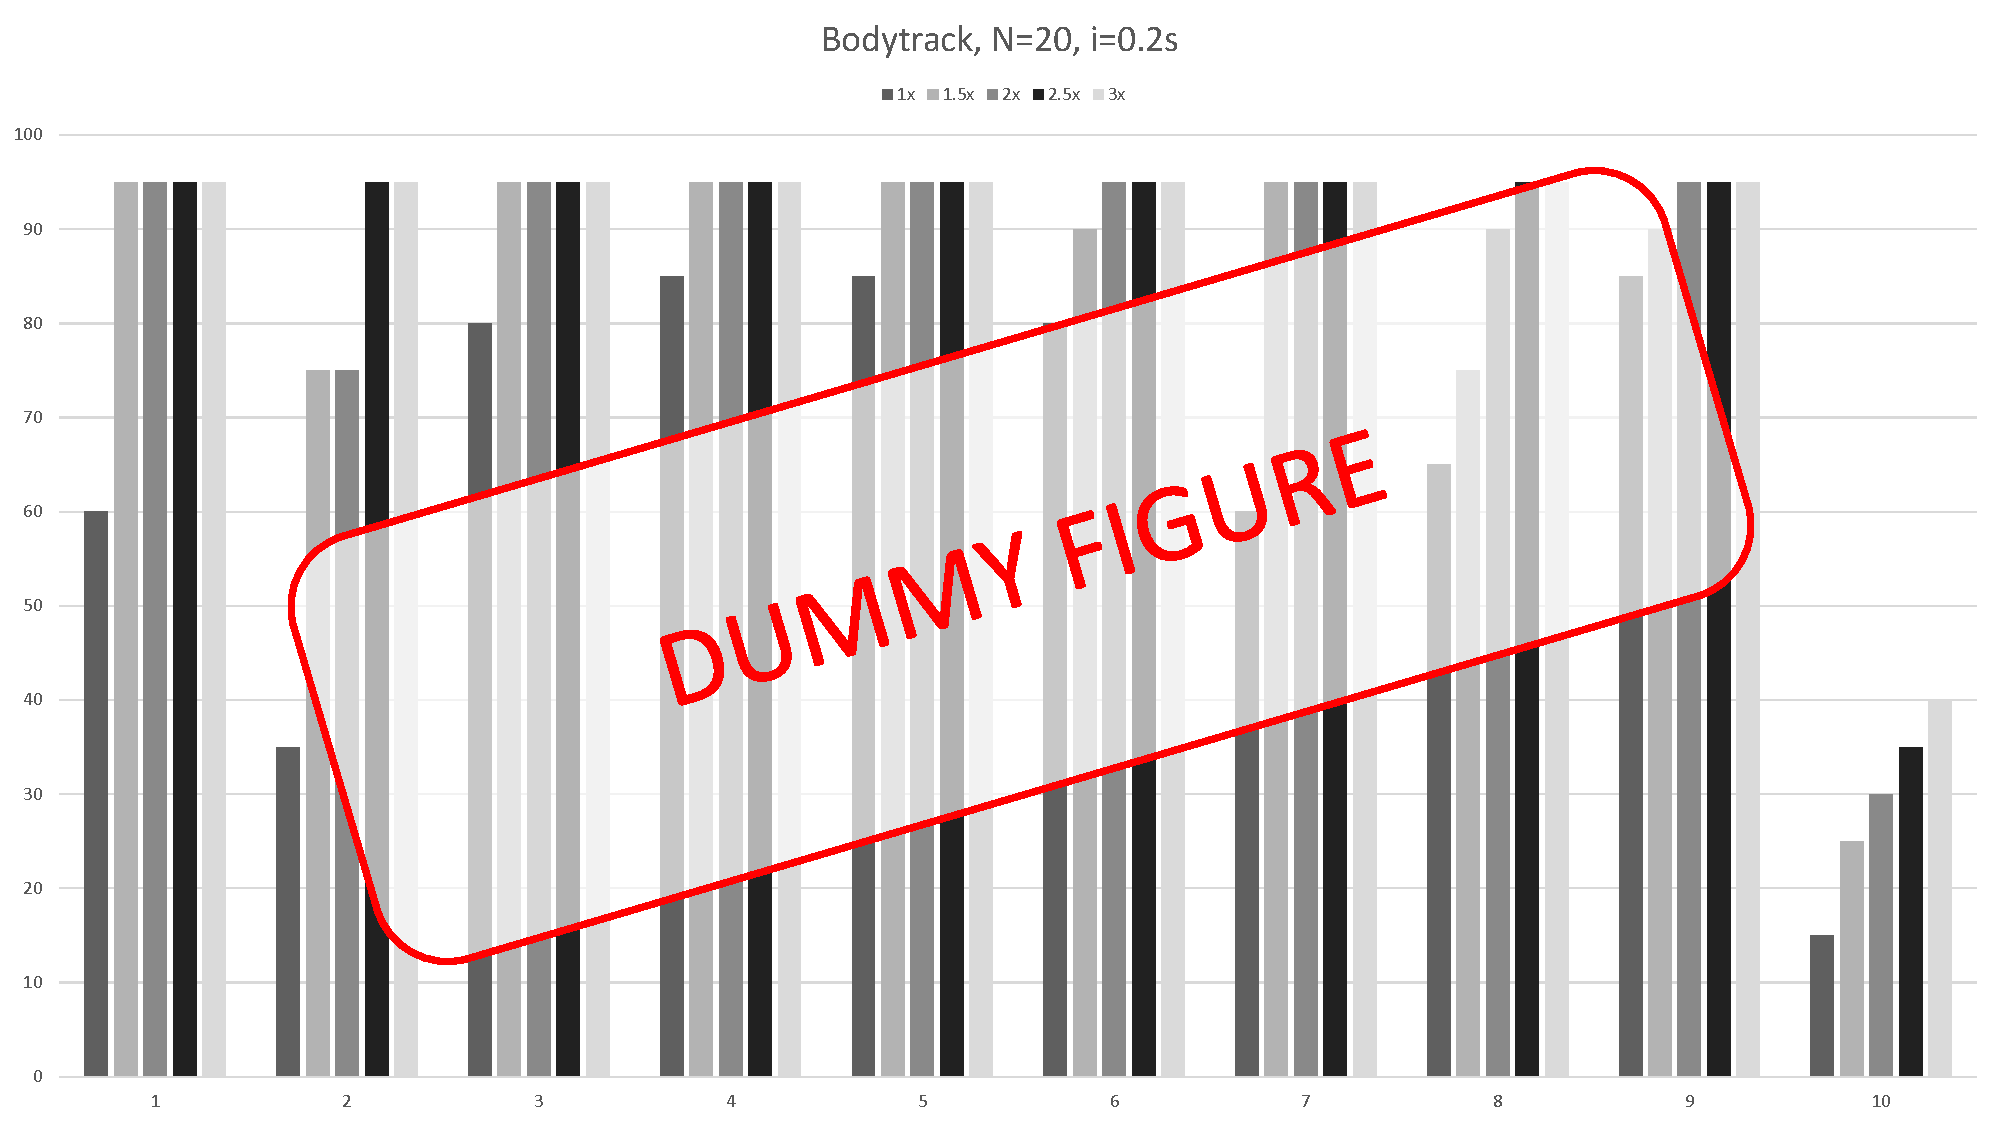
\includegraphics[width=0.46\textwidth]{figures/dummy.pdf}
  \caption{Remap design that allows re-migration}
  \label{fig:correct_remap}
\end{figure}


\subsection{Activity Tracking Mechanism}
\label{sec:tracking}


\subsection{Migration triggers}
Deciding when to perform migration is as important as knowing which pages to migrate. Migration adds a significant delay to a system and as such it must be used wisely. Any penalties incurred whould be amortised by the performance improvement when placing a page in the fast memory. Requests that arrive while migration is performed have to be delayed to ensure functionaly correct behavior. Two very common triggers are used throughout the literature whenever state must be updated based on tracking information (such as MC scheduling, NUMA, DVFS etc.). Interval-based (or epoch-based) triggers occur with a steady frequency, while threshold-based solutions trigger without a predetermined frequency, whenever a threshold value is passed. 

Both interval-based and threshold-based approaches face the same challenge of identifying the optimal interval or threshold value. Identifying the appropriate value is not usually a trivial task. Factors like a system's architecture, application's behavior, as well as semi-random factors (for example DRAM will refresh more frequently under higher temperatures) make the optimal value differ from system to system. Designers usually opt for the value that provides the best results on average. The optimal value should not be too small since it will trigger some potentially expensive procedure frequently, but it cannot be too large since that usually leads to potential performance loses. 

As far as memory migration in flat address spaces is concerned, the state-of-the-art mechanisms trigger their migration procedures based on:
\begin{enumerate}
	\item \textbf{THM approach:} THM uses a threshold-based mechanism. When the competing counter described in section \ref{sec:tracking} exceeds a threshold value, migration is triggered. THMwill swap the page that triggered the event with the page currently residing in the segment's fast memory page. As a result, a small chance exists that a cold page was accessed at the right time to trigger migration and now it resides in fast memory. Such a mistake should be quickly get resolved however, since the cold page in fast memory should get remigrated soon enough. \TODO{Check if they studied that effect.} THM's authors identified the optimal threshold value as \TODO{XX}.
	\item \textbf{HMA approach:} HMA uses an interval based mechanism. Upon each interval, HMA attempts to migrate as many pages in order to fill the fast memory. However with the high cost associated with the OS's intervention, management and the penalties of cold TLB force the interval value to be much larger. HMA authors identified the optimal timing interval to be as high as 1ms. \TODO{VERIFY}.
	\item \textbf{MemPod approach}: MemPod uses timing intervals. Like HMA, MemPod tried to fill the fast memory with hot pages on each interval. However, MemPod is transparent to the system and as such the need for costly OS intervention is waived. With the cost of a migration cycle kept to lower values, MemPod offers the possibility of a smaller interval time, which could potentially result in better performance. The optimal interval value is evaluated in the results section.
\end{enumerate}

\subsection{Migration Cost}

\subsection{Scalability to Future Memory Capacities}

\subsection{Discussion and comparison}
\TODO{Talk about limits in the size of remap tables/counters just fr the sake of argument. How would each mechanism handle it?}


















































